\pgfdeclarelayer{background}
\pgfsetlayers{background,main}

\colorlet{circle edge}{black!50}
\colorlet{circle area}{gray!20}

\def\network{{(0.1, -0.5)/-}, {(0.3, -1)/a}, {(0.7, -1.5)/b}, {(1.2, -2)/c}, {(1.8, -2)/e}, {(2.3, -1.5)/f}, {(2.7, -1)/g}, {(2.9, -0.5)/h}, {(1, -0.5)/i}, {(2, -0.5)/j}}
\def\connect{s/-, -/a, a/b, b/c, c/e, e/f, f/g, g/h, h/t}
\def\connectExtra{-/i, j/h}

\tikzset{
  filled/.style={fill=circle area, draw=circle edge, thick},
  outline/.style={draw=circle edge, thick}
  }

\setlength{\parskip}{5mm}

\tikzstyle{edge} = [draw, thick, -]
\tikzstyle{vertex}=[circle,fill=black!25,minimum size=10pt,inner sep=0pt]
\tikzstyle{invis-vertex}=[circle,fill=white!100,minimum size=0pt, inner sep=0pt]

\tikzstyle{selected edge} = [draw, line width=5pt,-,gray!50]
\tikzstyle{edge} = [draw, thick, -]

\subfloat[Initial deployment]{\label{fig:better_route1}
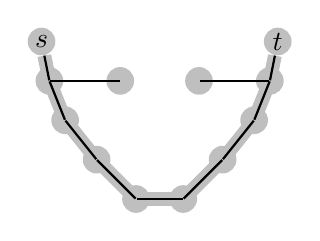
\begin{tikzpicture} 
  % The source and the sink, and the new node
  \foreach \pos/\name in {{(0,0)/s}, {(3, 0)/t}} {
    \node[vertex] (\name) at \pos {$\name$};
  }
         
  % The rest of the nodes
  \foreach \pos/\name in \network {
    \node[invis-vertex] (\name) at \pos {};
    \node[vertex] () at \pos {};
  }

  \begin{pgfonlayer}{background}
    \foreach \source/ \dest in \connect
      \path[selected edge] (\source) -- (\dest);
  \end{pgfonlayer}

  % All the connections but i and j
  \foreach \source/\sink in \connect
    \path[edge] (\source) -- (\sink);
       
  \foreach \source/\sink in \connectExtra
    \path[edge] (\source) -- (\sink);
\end{tikzpicture}}
% Remove empty line
\subfloat[New node added]{\label{fig:better_route2}
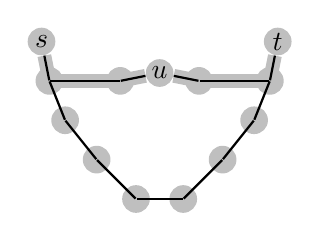
\begin{tikzpicture} 
  % The source and the sink, and the new node
  \foreach \pos/\name in {{(0,0)/s}, {(3, 0)/t}, {(1.5, -0.4)/u}} {
    \node[vertex] (\name) at \pos {$\name$};
  }
         
  % The rest of the nodes
  \foreach \pos/\name in \network {
    \node[invis-vertex] (\name) at \pos {};
    \node[vertex] () at \pos {};
  }

  \begin{pgfonlayer}{background}
    \foreach \source/ \dest in {s/-, -/i, i/u, u/j, j/h, h/t}
      \path[selected edge] (\source) -- (\dest);
  \end{pgfonlayer}

  % All the connections but i and j
  \foreach \source/\sink in \connect
    \path[edge] (\source) -- (\sink);
       
  \foreach \source/\sink in \connectExtra
    \path[edge] (\source) -- (\sink);
       
  \foreach \source/\sink in {i/u, u/j}
    \path[edge] (\source) -- (\sink);

\end{tikzpicture}}
